\section*{Exercício 7}

\begin{figure}[H]
    \center
    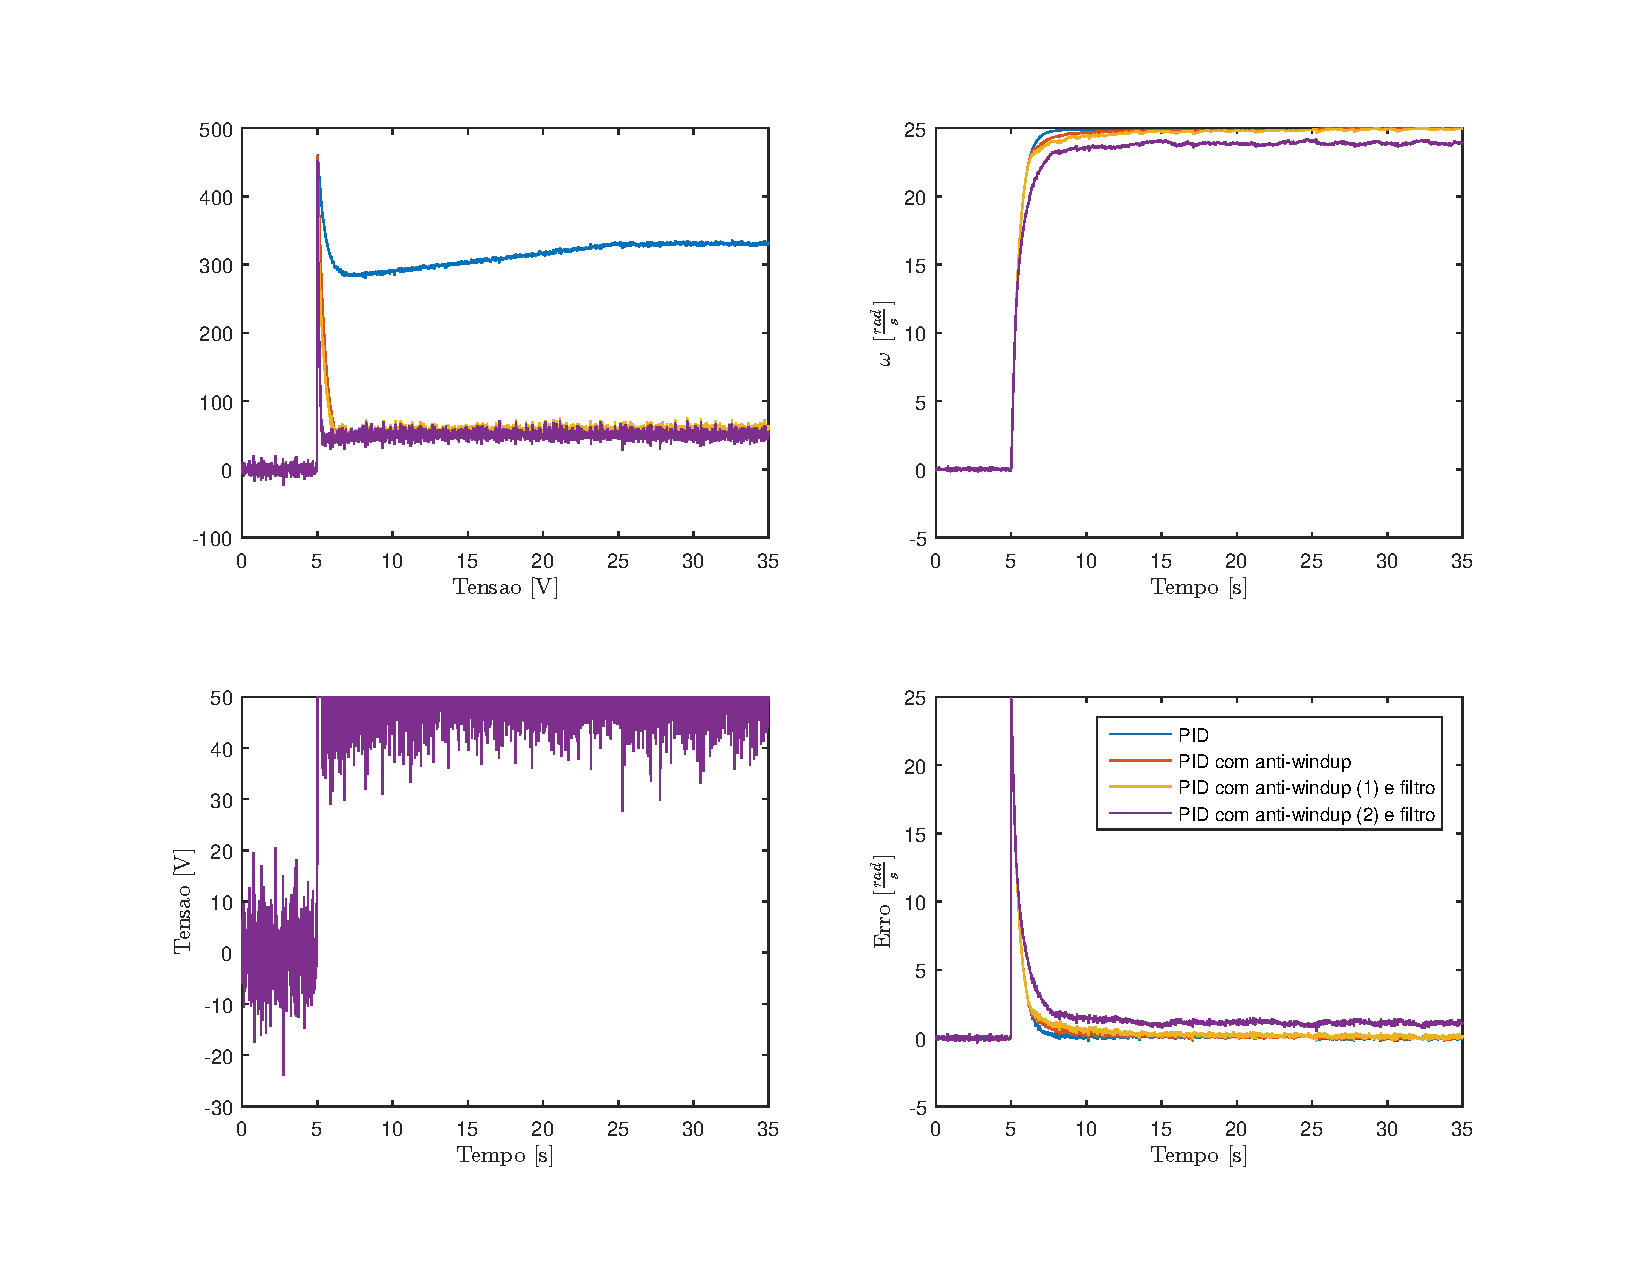
\includegraphics[width=1.2\textwidth, trim=4cm 2cm 1cm 1cm]{ex7.pdf}
    \caption{Principais sinais de controle do diagrama \ref{fig:dcIntrocomplete}}
    \label{fig:ex7}
\end{figure}

\begin{figure}[H]
    \center
    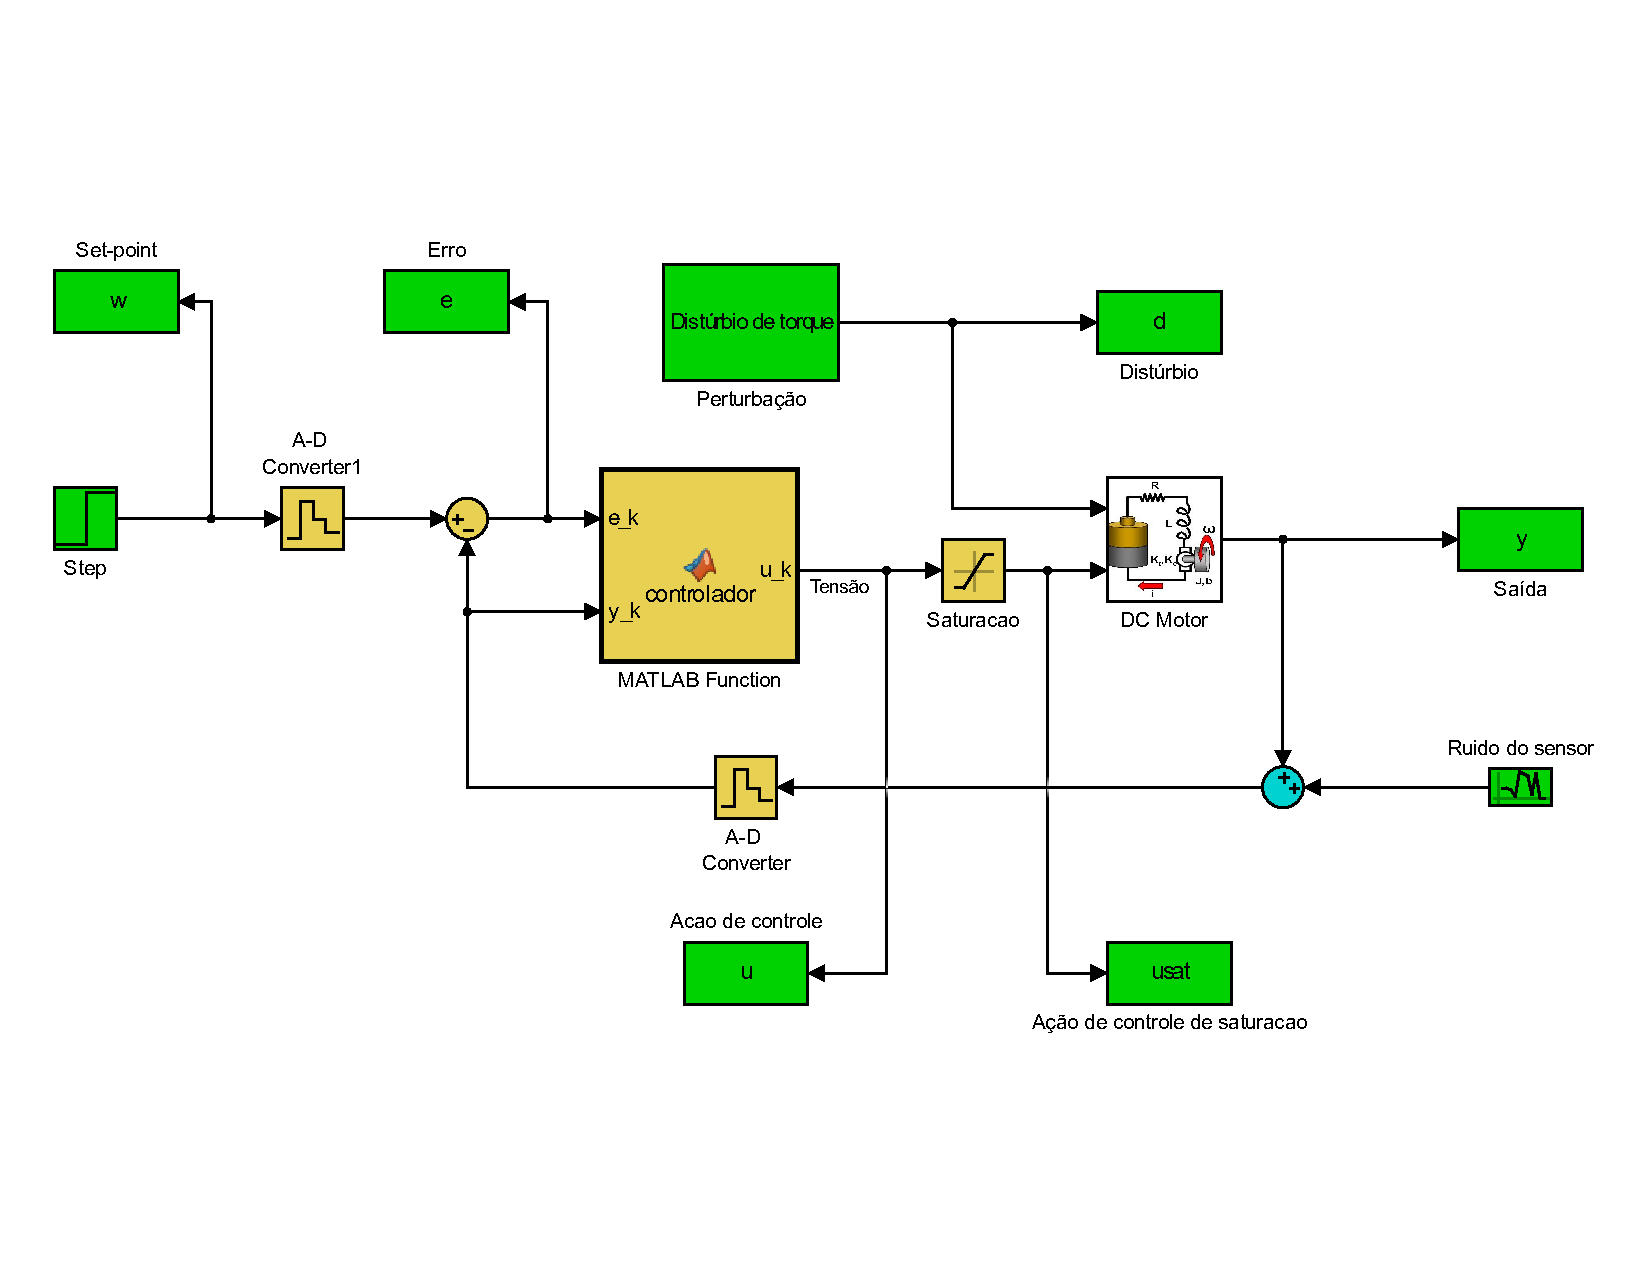
\includegraphics[width=0.8\textwidth, trim=3.5cm 3.5cm 2cm 2cm]{dcIntrocomplete.pdf}
    \caption{Diagrama de blocos utilizado para exercício 7}
    \label{fig:dcIntrocomplete}
\end{figure}

